\chapter{}

\titleimg{birdhead}

\mktitle{Capitulum Duodecimum}
\thispagestyle{empty}

\vnum{1}Dīxit quoque Dominus ad Moysēn et Aarōn in terrā
Ægyptī: \vnum{2}``Mēnsis iste, vōbīs prīncipium mēnsium: prīmus erit in mēnsibus
annī. \vnum{3}Loquiminī ad ūniversum \mpp{coetum:}{???}\mimg{babygoat}{haedus, -ī (m)}cœtum fīliōrum Isrāēl, et
dīcite eīs: Decima diē mēnsis huius tollat ūnusquisque agnum per familiās
et domōs suās. \vnum{4}Sīn autem minor est numerus ut \mpp{sufficere:}{satis esse}sufficere
possit ad \mpp{vēscī:}{ēdere}vēscendum agnum, assūmet \mpp{vicinus/a/um:}{prope habitans}vīcīnum suum quī iūnctus est domuī suæ, iuxtā numerum
animārum quæ sufficere possunt ad ēsum agnī.''

\vnum{5}``Erit autem agnus absque
\mpp{macula, -ae (f):}{pars in quā proprius color abest}maculā,
\mpp{masculus/a/um:}{masculīnus}masculus, \mpp{anniculus/a/um:}{unius annī}anniculus:
iuxtā quem \mpp{rītus, -ūs (m):}{res agendae ut sacra recte fiant}rītum
tollētis et hædum. \vnum{6}Et
servābitis eum usque ad quartamdecimam diem mēnsis huius:
\mpp{immolare:}{sacrificium facere}immolābitque eum ūniversa multitūdō
fīliōrum Isrāēl ad \mpp{vespera, -ae (f) =}{vesper}vesperam.''

\begin{figure}[h!]
    \begin{minipage}[hp]{0.5\linewidth}
        \centering
        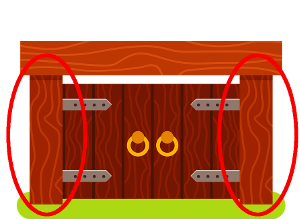
\includegraphics{postis}
        \caption{postis, -is (m)}
    \end{minipage}%
    \begin{minipage}[hp]{0.5\linewidth}
        \centering
        
\includegraphics{superlimen}
        \caption{superlīmināre, -is (n)}
    \end{minipage}
\end{figure}

\vnum{7}``Et sūment dē sanguine eius,
ac pōnent super utrumque postem, et in
superlīmināribus \mimg{lactuca}{lactūca, -ae (f)}domōrum, in quibus \mpp{comedere:}{totum
esse; esse}comedent illum. \vnum{8}Et edent carnēs nocte illa
\mpp{assus/a/um}{sine aquā vel aliā materiā fluentī coctus}assās ignī, et
\mpp{azȳmus/a/um:}{sine materiā quae efficit ut panis turgidus fiat}azȳmōs pānēs cum lactūcīs \mpp{agrestis, -e (adj):}{ad agros pertinens; rudis}agrestibus. \vnum{9}Nōn
comedētis ex eō \mpp{crūdus/a/um:}{non coctus}crūdum quid, nec coctum aquā, sed tantum
assum ignī: caput cum pedibus eius et intestīnīs
vorābitis.''

\begin{figure}[h!]
    \begin{minipage}[hp]{0.5\linewidth}
        \centering
        
\includegraphics{intestine}
        \caption{intestīnus, -ī (m)}
    \end{minipage}%
    \begin{minipage}[hp]{0.5\linewidth}
        \centering
        
\includegraphics{renes}
        \caption{rēnēs, rēnum (m)}
    \end{minipage}
\end{figure}

\vnum{10}``Nec remanēbit quidquam ex eō usque manē; sī quid
\mpp{residuus:}{quod reliquum est}residuum fuerit, igne
\mpp{comburere:}{igne perdere}combūrētis. \vnum{11}Sīc autem comedētis illum:
\mpp{rēnēs accingere:}{induere vestis quae cingit corpus circiter rēnēs}rēnēs vestrōs \mpp{accingere =}{cingere}accingētis, et
\mpp{calceamentum:}{quod pedi induitur}calceāmenta habēbitis in pedibus,
tenentēs baculōs in manibus, et comedētis \mpp{festīnanter =}{celeriter}festīnanter: est
enim \mpp{Phase:}{vocabulum Hebraicum ``trānsitus'' significans}Phase (id est, trānsitus) Dominī. \vnum{12}Et trānsībō per
terram Ægyptī nocte illa, percutiamque omne \mpp{prīmōgenitus/a/um:}{quī vel quae prīmus natus est}prīmōgenitum in
terrā Ægyptī ab homine usque ad pecūs: et in cūnctīs dīīs Ægyptī faciam
\mpp{iūdicium, -ī (n):}{quod iudex tradit}\mimg{judge_small}{iudex, iudicis (m/f)}iūdicia. Ego Dominus. \vnum{13}Erit autem sanguis vōbīs in signum
in \mpp{aedēs, aedium (f pl.):}{aedificium}ædibus in quibus eritis: et vidēbō sanguinem, et
trānsībō vōs: nec erit in vōbīs \mpp{plāga, -ae (f):}{e.g, unus pulsat alterum eo
tempore cum pugnus corpus tangit `plāga' vocatur}plāgā
\mpp{disperdere:}{valde perdere}disperdēns quandō percusserō terram Ægyptī. \vnum{14}Habēbitis
autem hunc diem in \mpp{monumentum, -ī (n):}{quiquid nōs monet}monumentum: et
\mpp{celebrāre:}{agere quod oportet agere die Deō pertinentī}celebrābitis eam \mpp{sōlemnis, -e (adj):}{dicitur de rēbus deō pertinentibus quae certīs temporibus quotannis fit}sōlemnem Dominō in
\mpp{????}{????}generātiōnibus vestrīs cultū \mpp{sempiternus/a/um:}{perpetuus}sempiternō.
\vnum{15}Septem diēbus azȳma comedētis: in diē prīmō nōn erit
\mpp{fermentum, -ī (n):}{materia quae efficit ut panis turgidus fiat}fermentum in domibus vestrīs: quīcumque comēderit
\mpp{fermentō, -āre, -āvī, -ātum:}{ponere fermentum in aliquō}fermentātum, perībit anima illa dē Isrāēl, ā prīmō diē
usque ad diem septimum.''

\vnum{16}``Diēs prīma erit \mpp{sānctus/a/um:}{deō pertinens}sāncta atque
sōlemnis, et diēs septima eādem \mpp{fēstīvitās, -ātis (f):}{mos diebus solemnibus}fēstīvitāte
\mpp{venerābilis, -e (adj):}{cultū dignus}venerābilis: nihil operis faciētis in eīs,
\mpp{exceptīs hīs:}{praeter hās}exceptīs hīs, quæ ad vēscendum \mpp{pertinere:}{e.g,
colloquium ad me pertinet si homines loquuntur de me}pertinent. \vnum{17}Et
\mpp{observābitis azȳma:}{quotannis diem sanctam celebrētis in quā azymī panēs comeduntur}observābitis azȳma: in eādem enim ipsā diē ēdūcam
exercitum vestrum dē terrā Ægyptī, et cūstōdiētis diem istum in
\mpp{generātio, -ōnis (f):}{e.g: una generatio parentibus constat, līberīs eōrum altera generatio constat, etc...}generātiōnēs vestrās \mpp{rītus, -ūs (m):}{res agendae ut sacra recte fiant}rītū perpetuō.  \vnum{18} Prīmō mēnse, quartadecīmā diē mēnsis ad vesperam, comedētis
azȳma usque ad diem \mpp{vīgēsimam =}{vīcēsimam}vīgēsimam prīmam eiusdem mēnsis ad
vesperam. \vnum{19}Septem diēbus fermentum nōn inveniētur in domibus vestrīs:
quī comēderit fermentātum, perībit anima eius dē cœtū Isrāēl, tam dē
\mpp{advena, -ae (m)}{qui non est civis, qui ab alio loco venit}advenīs quam dē \mpp{indigena, -ae (adj)}{natus in eō lōcō}indigenīs terræ. \vnum{20}Omne fermentātum nōn
comedētis: in cūnctīs \mpp{habitāculum, -ī (n):}{locus in quō aliquis habitat}habitāculīs vestrīs edētis azȳma.''

\vnum{21}Vocāvit autem Moysēs omnēs seniōrēs fīliōrum Isrāēl, et
dīxit ad eōs: ``Īte tollentēs animal per familiās vestrās, et immolātē
Phase. \vnum{22}\mpp{fasciulum, -ī:}{multum lignī vel materiae aliae vinctum}Fasciculumque \mpp{hyssōpum, -ī (n):}{herba quaedam}hyssōpī
\mpp{tingere:}{humidum facere}tingite in sanguine quī est in līmine, et aspergite ex eō
superlīmināre, et utrumque postem: nūllus vestrum
ēgrediātur ōstium domūs suæ usque manē. \vnum{23}Trānsībit enim Dominus
percutiēns Ægyptiōs: cumque vīderit sanguinem in
superlīminārī, et in utrōque poste,
\mpp{trānscendere:}{transīre}trānscendet ōstium domūs, et nōn sinet
\mpp{percussōr, -ōris (m):}{quī percutit}percussōrem \mpp{ingredi:}{intus ire}ingredī domōs vestrās
et lædere. \vnum{24}Cūstōdī verbum istud \mpp{lēgitimus/a/um:}{qui secundum legēs est; iustus; verus}lēgitimum tibi et fīliīs
tuīs usque in \mpp{in aeternum:}{semper}æternum. \vnum{25}Cumque \mpp{introire:}{intus ire;
ingredi}introierītis terram, quam Dominus datūrus est vōbīs ut pollicitus
est, observābitis \mpp{cæremōnia, ae (f):}{res agendae ut sacra recte fiant}cæremōniās istās. \vnum{26}Et cum dīxerint
vōbīs fīliī vestrī: Quæ est ista \mpp{religiō, -ōnis (f):}{rītus}religiō? \vnum{27}Dīcētis eīs:
\mpp{victima, -ae (f):}{animal sacrificiō statutum}Victima trānsitūs Dominī est, quandō trānsīvit super
domōs fīliōrum Isrāēl in Ægyptō, percutiēns Ægyptiōs, et domōs nostrās
līberāns.''

\mimg{scimitar}{gladius \emph{incurvātus}}Incurvātusque populus adōrāvit. \vnum{28}Et ēgressī
fīliī Isrāēl fēcērunt sīcut \mpp{praecipere:}{imperare}præcēperat Dominus
Moȳsī et Aarōn. \vnum{29}Factum est autem in noctīs mediō, percussit Dominus omne
\mpp{prīmōgenitus/a/um:}{quī vel quae prīmus natus est}prīmōgenitum in terrā Ægyptī, ā prīmōgenitō
Pharaōnis, quī in soliō eius sedēbat, usque ad prīmōgenitum
\mpp{captīvus/a/um:}{qui captus, qui vinctus est}captīvæ quæ erat in carcere, et omne prīmōgenitum
\mpp{iumentum:}{animal utile ad gerendum vel trahendum e.g, equi, boves, et
cetera}iūmentōrum. \vnum{30}Surrēxitque Pharaō nocte, et omnēs
servī eius, cūnctaque Ægyptus: et ortus est clāmor magnus in Ægyptō:
neque enim erat domus in quā nōn iacēret mortuus. 

\vnum{31}Vocātīsque Pharaō
Moyse et Aarōn nocte, ait: ``Surgite et ēgrediminī ā populō
meō, vōs et fīliī Isrāēl: īte, immolātē Dominō sīcut dīcitis. \vnum{32}Ovēs
vestrās et \mpp{armentum, -ī (n):}{maiorum bestiarum grex (e.g: equōrum, bovum)}armenta assūmite ut petierātis, et abeuntēs
\mpp{benedīcere:}{sanctum facere}benedīcite mihi.''

\vnum{33}\mpp{urgēre:}{valde hortārī; cogere}Urgēbantque Ægyptiī
populum dē terrā exīre vēlōciter, dīcentēs: ``Omnēs moriēmur.''

\vnum{34}Tulit
igitur populus \mpp{cōnspergō, cōnspergere, cōnspersī, conspersum:}{spargere}cōnspersam \mpp{farīna, -ae (f):}{materia, aquā impositā, ex quā panis factus est}farīnam antequam
\mpp{fermentō, -āre, -āvī, -ātum:}{ponere fermentum in aliquō}fermentārētur: et ligāns in palliīs, posuit super
\mpp{humerōs =}{umerōs}humerōs suōs. \vnum{35}Fēcēruntque fīliī Isrāēl sīcut præcēperat
Moysēs: et petiērunt ab Ægyptiīs vāsa argentea et aurea, vestemque
plūrimam. \vnum{36}Dominus autem dedit grātiam populō cōram Ægyptiīs ut
\mpp{commodāre:}{libenter cum aliquō facere, libenter rēs dāre}commodārent eīs: et \mpp{spoliare:}{capere res aliorum
hominum}spoliāvērunt Ægyptiōs. 

\vnum{37}Profectīque sunt fīliī Isrāēl dē Ramesse
in Socoth, sexcenta ferē mīllia peditum virōrum, absque parvulīs. \vnum{38}Sed et
\mpp{vulgus, -ī (n):}{multitudo, turba}vulgus \mpp{prōmiscuus/a/um:}{mixtum}prōmiscuum \mpp{innumerabilis:}{qui
numerari non potest}innumerābile ascendit cum eīs, ovēs et armenta et
animantia \mpp{diversus:}{in varias partes versi sunt}dīversī generis multa
nimis. \vnum{39}Coxēruntque farīnam, quam \mpp{dūdum:}{nuper}dūdum dē Ægyptō
cōnspersam tulerant: et fēcērunt \mpp{subcinerīcus pānis:}{panis sub cinere coctus}subcinerīciōs pānēs
azȳmōs: neque enim poterant fermentārī, cōgentibus exīre
Ægyptiīs, et nūllam facere sinentibus moram: nec \mpp{pulmentum, -ī (n):}{cibus}pulmentī
quidquam occurrerat \mpp{praeparāre:}{parāre, ante parāre}præparāre.

\vnum{40}\mpp{habitātiō, -ōnis (f)}{actus habitandī}Habitātiō
autem fīliōrum Isrāēl quā mānsērunt in Ægyptō, fuit quadringentōrum
trīgintā annōrum. \vnum{41}Quibus \mpp{explere:}{perficere}explētīs, eādem diē
ēgressus est omnis exercitus Dominī dē terrā Ægyptī. \vnum{42}Nox ista est
\mpp{???}{???}observābilis Dominī, quandō ēdūxit eōs dē terrā Ægyptī: hanc
observāre dēbent omnēs fīliī Isrāēl in generātiōnibus suīs.

\vnum{43}Dīxitque Dominus ad Moysēn et Aarōn: ``Hæc est religiō Phase: omnis
\mpp{aliēnigena, -ae (m/f):}{aliō locō natus}aliēnigena nōn comedet ex eō. \vnum{44}Omnīs autem servus
\mpp{emptitius =}{emptus}emptitius \mpp{circumcīdere:}{Removēre secandō summum membrum inter crura puerī vel virī situm}circumcīdētur, et sīc comedet. \vnum{45}Advena et
\mpp{mercēnārius, -ī (m):}{cui merces datur ut opus faciat}mercēnārius nōn edent ex eō. \vnum{46}In ūnā domō comedētur, nec
\mpp{efferre:}{extra ferre, proferre}efferētis dē carnibus eius forās, nec os illīus
\mpp{confringere:}{una frangere}cōnfringētis. \vnum{47}Omnīs cœtūs fīliōrum
Isrāēl faciet illud. \vnum{48}Quod sī quis \mpp{peregrīnus/a/um:}{quī ex aliā terrā vēnit}peregrīnōrum in
vestram voluerit trānsīre \mpp{colōnia, -ae (f):}{locus in quō hominēs domūs novās confēcērunt et agrōs colere incēpērunt}colōniam, et facere Phase Dominī,
circumcīdētur prius omne masculīnum eius, et tunc \mpp{rītus, -ūs (m):}{res agendae ut sacra recte fiant}rīte
celebrābit: eritque sīcut \mpp{indigena, -ae (adj)}{natus in eō lōcō}indigena terræ:
sī quis autem circumcīsus nōn fuerit, nōn
\mpp{vēscī:}{ēdere}vēscētur ex eō. \vnum{49}Eādem lēx erit indigenæ
et colōnō quī \mpp{peregrinārī:}{iter facere per aliēna loca, patria procul abīre}peregrīnātur apud vōs.''

\vnum{50}Fēcēruntque omnēs
fīliī Isrāēl sīcut præcēperat Dominus Moȳsī et Aarōn. \vnum{51}Et eādem diē
ēdūxit Dominus fīliōs Isrāēl dē terrā Ægyptī per \mpp{turma, -ae (f):}{multitūdō}turmās
suās. 
